\documentclass[letterpaper]{article}
\usepackage[margin=1in]{geometry}

% Set the typeface to Times Roman
\usepackage{times}

%\usepackage{hyperref}
\usepackage{amsfonts}%
\usepackage{amssymb}%
\usepackage{amsthm}% allows theoremstyles (see below) and provides a proof environment
\usepackage{bm}
\usepackage{relsize}
\usepackage{graphicx}
\usepackage{caption}
\usepackage{epstopdf}
\usepackage{amsmath}
\usepackage{tikz}
\usetikzlibrary{trees,arrows}
\usepackage{cite}
\usetikzlibrary{decorations}
\usetikzlibrary[decorations]
\usepgflibrary{decorations.pathmorphing}
\usepgflibrary[decorations.pathmorphing]
\usetikzlibrary{decorations.pathmorphing}
\usetikzlibrary[decorations.pathmorphing]
\usepackage{booktabs}
\usepackage[authoryear]{natbib}
\usepackage{subcaption}
\usepackage{pseudocode}
%\usepackage{float}
\usepackage{verbatim} %% for commenting blocks

\bibpunct{(}{)}{,}{}{}{;} %% added this to make \citep{x} use parentheses

%% independence symbol and expectation operator %%
\newcommand\independent{\protect\mathpalette{\protect\independenT}{\perp}}
\def\independenT#1#2{\mathrel{\rlap{$#1#2$}\mkern2mu{#1#2}}}

\DeclareMathOperator*{\E}{\mathbb{E}}
\DeclareMathOperator*{\Et}{\mathbb{E}_t}
\DeclareMathOperator*{\argmax}{arg\,max}
\DeclareMathOperator{\circlearrow}{\hbox{$\circ$}\kern-1.5pt\hbox{$\rightarrow$}}
\DeclareMathOperator{\circlecircle}{\hbox{$\circ$}\kern-1.2pt\hbox{$--$}\kern-1.5pt\hbox{$\circ$}}

\newcommand\indep{\protect\mathpalette{\protect\independenT}{\perp}}
\def\independenT#1#2{\mathrel{\rlap{$#1#2$}\mkern2mu{#1#2}}}

\newtheorem{Lma}{Lemma}
\newtheorem{Thm}{Theorem}

\DeclareMathOperator*{\Pa}{\text{Pa}}
\DeclareMathOperator*{\Ne}{\text{Ne}}
\DeclareMathOperator*{\Adj}{\text{Adj}}
\DeclareMathOperator*{\Ch}{\text{Ch}}
\DeclareMathOperator*{\An}{\text{An}}
\DeclareMathOperator*{\De}{\text{De}}
\DeclareMathOperator*{\Sp}{\text{Sp}}
\DeclareMathOperator*{\Si}{\text{Si}}
\DeclareMathOperator*{\Nd}{\text{Nd}}
\DeclareMathOperator*{\Mb}{\text{Mb}}
\DeclareMathOperator*{\Cl}{\text{Cl}}
\DeclareMathOperator*{\Bd}{\text{Bd}}

%%%%%%%%%%%%%%%%%%%%%%%%%%%%

\title{Assignment 3}

\author{}

\date{Due: October 25th at 8pm EST}

\begin{document}

\maketitle

	Instructions: This is an individual assignment, not group work. Though you may
	discuss the problems with your classmates, you must solve the problems and
	write the solutions independently. As stated in the syllabus, copying code
	from a classmate or the internet (even with minor changes) constitutes
	plagiarism. You are required to submit your answers in pdf form (use \LaTeX)
	in a file called \texttt{<your-UNI>-hw3.pdf} to courseworks. 
	The code for the programming assignment should be appended at the end of this pdf.
	Late submissions will be penalized, except in extenuating circumstances such
	as medical or family emergency. Submissions submitted 0-24 hours late will be
	penalized 10\%, 24-48 hours late by 20\%, 48-72 hours late by 30\%, and later
	than 72 hours by 100\% (i.e., zero credit). Each question is worth 5 points, for a total of 25 points.

\section*{Problem 1}

Let $X \sim N(\mu, \Sigma)$ where $X = (X_1,...,X_p)$. We saw in class that marginal independence in the multivariate normal model corresponds to zeros in the covariance matrix, i.e., $X_i \independent X_j$ if and only if $\Sigma_{ij} = 0$. We also saw that conditional independence where the conditioning set is ``everything else'' corresponds to zeros in the precision matrix: $X_i \independent X_j | X \setminus\{X_i,X_j\}$ if and only if $K_{ij}=0$. Let $X_S \subset X\setminus\{X_i,X_j\}$ be some arbitrary subset of the variables. Explain why the following is true: $X_i \independent X_j | X_S $ if and only if $( \Sigma_{\{ijS\},\{ijS\} } )^{-1}_{ij} = 0$ (Hint: that conditional independence statement amounts to a marginal independence $X_i \independent X_j$ in the conditional distribution where $X_S = x_S$. What is that conditional distribution?)

\section*{Problem 2}

Use the following code to simulate data from a given MRF independence model:
\begin{verbatim}
set.seed(123)
( K <- cbind(c(10,7,7,0),c(7,20,0,7),c(7,0,30,7),c(0,7,7,40)) )
data <- as.data.frame(mvrnorm(n=10000,mu=c(0,0,0,0),Sigma=solve(K)))
colnames(data) <- c("X1","X2","X3","X4")
\end{verbatim}
(Note: in R, the inverse of a matrix \texttt{M} is obtained by \texttt{solve(M)}.) What are the conditional independencies that are representing in this precision matrix? What is the corresponding graph? Verify the conditional independence constraints by using linear regression. Explain all this.

\noindent Next, use the \texttt{gRim} package to fit the model, i.e., estimate the precision matrix subject to the graph constraints.
\begin{verbatim}
library(gRim)
glist <- list( *insert list of edges here* )
ddd <- cov.wt(data, method="ML")
fit <- ggmfit(ddd$cov, ddd$n.obs, glist) # Estimate parameters using IPF
fit$K # estimated precision matrix
\end{verbatim}

\noindent Did it work? How do you know?

\section*{Problem 3}

Consider the Gaussian Bayesian Network model with the following covariance matrix:
\begin{verbatim}
set.seed(123)
( Sig <- cbind(c(3,-1.4,0,0),c(-1.4,3,1.4,1.4),c(0,1.4,3,0),c(0,1.4,0,3)) )
data <- as.data.frame(mvrnorm(n=10000,mu=c(0,0,0,0),Sigma=Sig))
colnames(data) <- c("X1","X2","X3","X4")
\end{verbatim}
and the DAG $\mathcal{G}$ with edges $X_1 \rightarrow X_2 \leftarrow X_3$ and $X_4 \rightarrow X_2$.\\

\noindent a) What correlation constraints does this model represent? Estimate the correlation matrix.\\

\noindent b) Consider also the moralized graph $\mathcal{G}^m$ and what the corresponding precision matrix $K$ would look like. What are the partial correlation constraints represented in $K$? How does this make sense with respect to $\Sigma$ above? \\

\noindent c) Following steps similar to the previous problem, estimate the corresponding precision matrix $K$ from this data (using \texttt{ggmfit}). Take the inverse and compare to the true covariance matrix.

\section*{Problem 4}

Use \texttt{dagitty} to simulate 10000 observations from this graph:
\begin{verbatim}
g <- dagitty( "dag{ x <- u1; u1 -> m <- u2 ; u2 -> y }" )
\end{verbatim}
Here $U_1,U_2$ represent unmeasured variables. Estimate the effect of $X$ on $Y$ adjusting for $M$ in a linear regression, obtaining a 95\% confidence interval for the effect. Then estimate the same effect (and confidence interval) using the correct sufficient adjustment set that you can obtain from \texttt{dagitty}. What conclusion should be drawn from this example?

\section*{Problem 5}

Construct the DAG in Figure \ref{fig:prob6} as a daggity object. Simulate 10000 observations from this graph using \texttt{simulateSEM()} as you did on the first homework. Estimate the effect of $E$ on $F$ and the effect of $B$ on $A$ using backdoor adjustment and linear regression. If there is more than one sufficient adjustment set, try each of the ones identified by \texttt{dagitty} and compare them. Are the point estimates similar? Do the estimates have similar variance (or confidence interval length)? Compare also these estimates against an approach which simply adjusts for \emph{all} other variables in the graph. How are the results different (if they are) and what is the explanation?

\begin{figure}[h]
	\begin{center}
		\scalebox{0.7}{
			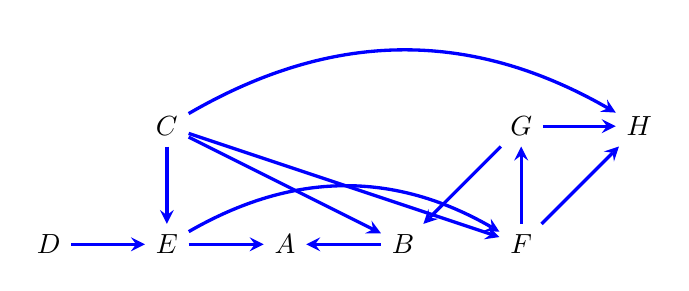
\begin{tikzpicture}[>=stealth, node distance=1.5cm]
			\tikzstyle{format} = [draw, thick, circle, minimum size=1.0mm, inner sep=0pt]
			\tikzstyle{square} = [draw, thick, minimum size=1.0mm, inner sep=3pt]
			\begin{scope}
			\path[->, very thick]
			node[] (C) {$C$}
			node[below of=C] (E) {$E$}
			node[right of=E] (A) {$A$}
			node[left of=E] (D) {$D$}
			node[right of=A] (B) {$B$}
			node[right of = B] (F) {$F$}
			node[above of = F] (G) {$G$}
			node[right of = G] (H) {$H$}
			(B) edge[blue] (A)
			(E) edge[blue] (A) 
			(C) edge[blue] (B)
			(F) edge[blue] (H)
			(D) edge[blue] (E)
			(C) edge[blue] (E)
			(C) edge[blue] (F)
			(C) edge[blue, bend left] (H)
			(G) edge[blue] (H)
			(F) edge[blue] (G)
			(G) edge[blue] (B)
			(E) edge[blue, bend left] (F)
			;
			\end{scope}
			\end{tikzpicture}
		}
	\end{center}
	\caption{}
	\label{fig:prob6}
\end{figure}


\end{document}
